%-------------------------------------------------------------------------------
%	PACKAGES AND OTHER DOCUMENT CONFIGURATIONS
%-------------------------------------------------------------------------------

\documentclass{article}

\usepackage{fancyhdr} % Required for custom headers
\usepackage{lastpage} % Required to determine the last page for the footer
\usepackage{extramarks} % Required for headers and footers
\usepackage[usenames,dvipsnames]{color} % Required for custom colors
\usepackage{graphicx} % Required to insert images
\usepackage{listings} % Required for insertion of code
\usepackage{courier} % Required for the courier font
\usepackage{lipsum} % Used for inserting dummy 'Lorem ipsum' text
\usepackage{amsmath}


% formatting
\pdfcompresslevel0

% ==============================================================================
% PYTHON
% ==============================================================================
\usepackage[utf8]{inputenc}

% Default fixed font does not support bold face
\DeclareFixedFont{\ttb}{T1}{txtt}{bx}{n}{12} % for bold
\DeclareFixedFont{\ttm}{T1}{txtt}{m}{n}{12}  % for normal

% Custom colors
\usepackage{color}
\definecolor{deepblue}{rgb}{0,0,0.5}
\definecolor{deepred}{rgb}{0.6,0,0}
\definecolor{deepgreen}{rgb}{0,0.5,0}

\usepackage{listings}

% Python style for highlighting
\newcommand\pythonstyle{\lstset{
language=Python,
basicstyle=\ttm,
otherkeywords={self},             % Add keywords here
keywordstyle=\ttb\color{deepblue},
emph={MyClass,__init__},          % Custom highlighting
emphstyle=\ttb\color{deepred},    % Custom highlighting style
stringstyle=\color{deepgreen},
frame=tb,                         % Any extra options here
showstringspaces=false,            % 
breaklines=true
}}


% Python environment
\lstnewenvironment{python}[1][]
{\pythonstyle\lstset{#1}
}
{}

% Python for external files
\newcommand\pythonexternal[2][]{{
\pythonstyle\lstinputlisting[#1]{#2}}}

% Python for inline
\newcommand\pythoninline[1]{{\pythonstyle\lstinline!#1!}}
% ==============================================================================
% ==============================================================================

% Margins
\topmargin=-0.45in
\evensidemargin=0in
\oddsidemargin=0in
\textwidth=6.5in
\textheight=9.0in
\headsep=0.25in

\linespread{1.1} % Line spacing

% Set up the header and footer
\pagestyle{fancy}
\lhead{\hmwkAuthorName} % Top left header
\chead{\hmwkClass\ (\hmwkClassInstructor\ \hmwkClassTime): \hmwkTitle} % Top center head
\rhead{\firstxmark} % Top right header
\lfoot{\lastxmark} % Bottom left footer
\cfoot{} % Bottom center footer
\rfoot{Page\ \thepage\ of\ \protect\pageref{LastPage}} % Bottom right footer
\renewcommand\headrulewidth{0.4pt} % Size of the header rule
\renewcommand\footrulewidth{0.4pt} % Size of the footer rule

\setlength\parindent{0pt} % Removes all indentation from paragraphs

%----------------------------------------------------------------------------------------
%	DOCUMENT STRUCTURE COMMANDS
%	Skip this unless you know what you're doing
%----------------------------------------------------------------------------------------

% Header and footer for when a page split occurs within a problem environment
\newcommand{\enterProblemHeader}[1]{\nobreak\extramarks{#1}{#1 continued on next page\ldots}\nobreak\nobreak\extramarks{#1 (continued)}{#1 continued on next page\ldots}\nobreak}

% Header and footer for when a page split occurs between problem environments
\newcommand{\exitProblemHeader}[1]{\nobreak\extramarks{#1 (continued)}{#1 continued on next page\ldots}\nobreak\nobreak\extramarks{#1}{}\nobreak}

\setcounter{secnumdepth}{0} % Removes default section numbers
\newcounter{homeworkProblemCounter} % Creates a counter to keep track of the number of problems

\newcommand{\homeworkProblemName}{}
\newenvironment{homeworkProblem}[1][Problem \arabic{homeworkProblemCounter}]{ % Makes a new environment called homeworkProblem which takes 1 argument (custom name) but the default is "Problem #"
\stepcounter{homeworkProblemCounter} % Increase counter for number of problems
\renewcommand{\homeworkProblemName}{#1} % Assign \homeworkProblemName the name of the problem
\section{\homeworkProblemName} % Make a section in the document with the custom problem count
\enterProblemHeader{\homeworkProblemName} % Header and footer within the environment
}{\exitProblemHeader{\homeworkProblemName} % Header and footer after the environment
}

% Defines the problem answer command with the content as the only argument
\newcommand{\problemAnswer}[1]{\noindent\framebox[\columnwidth, resolution=600][c]{\begin{minipage}{0.98\columnwidth, resolution=600}#1\end{minipage}}}
% Makes the box around the problem answer and puts the content inside }

\newcommand{\homeworkSectionName}{}
\newenvironment{homeworkSection}[1]{ % New environment for sections within homework problems, takes 1 argument - the name of the section
\renewcommand{\homeworkSectionName}{#1} % Assign \homeworkSectionName to the name of the section from the environment argument
\subsection{\homeworkSectionName} % Make a subsection with the custom name of the subsection
\enterProblemHeader{\homeworkProblemName\ [\homeworkSectionName]} % Header and footer within the environment
}{
\enterProblemHeader{\homeworkProblemName} % Header and footer after the environment
}



%----------------------------------------------------------------------------------------
%	NAME AND CLASS SECTION
%----------------------------------------------------------------------------------------

\newcommand{\hmwkTitle}{Final} % Assignment title
\newcommand{\hmwkDueDate}{Friday, May 16} % Due date
\newcommand{\hmwkClass}{Astron 702} % Course/class
\newcommand{\hmwkClassTime}{1:20 pm} % Class/lecture time
\newcommand{\hmwkClassInstructor}{Townsend} % Teacher/lecturer
\newcommand{\hmwkAuthorName}{Elijah Bernstein-Cooper} % Your name

%-------------------------------------------------------------------------------
%	TITLE PAGE
%-------------------------------------------------------------------------------

\title{\vspace{2in}
    \textmd{\textbf{\hmwkClass:\ \hmwkTitle}}\\
    \normalsize\vspace{0.1in}\small{Due\ on\ \hmwkDueDate}\\
    \vspace{0.1in}\large{\textit{\hmwkClassInstructor\ \hmwkClassTime}}
    \vspace{3in}}

\author{\textbf{Elijah Bernstein-Cooper}}
\date{\today} % Insert date here if you want it to appear below your name

%-------------------------------------------------------------------------------

\begin{document}

\maketitle
\newpage

%===============================================================================
%-------------------------------------------------------------------------------
%	PROBLEM 1
%-------------------------------------------------------------------------------
\begin{homeworkProblem}

    Using the Forward-Time Center-Space (FTCS) scheme to calculate the
    progression of $y(x,t)$ we use the following

    \begin{equation}
        y^{n+1}_k = y^n_k - a(t^{n+1} - t^{n})  \
        \frac{y^n_{k+1} - y^n_{k-1}}{x_{k+1} - x_{k-1}}
    \end{equation}
   
    We use this scheme to calculate $y(x,t)$ on the intervals $0 < x < 1$ and
    $0 < t < 3$ with $\delta x = 0.01$ and $\delta t = 0.005$ with periodic
    boundary conditions. After running this simulation we find that the FTCS
    scheme reproduces the analytic result of 
    
    \begin{equation} \label{eq:y}
        y(x,t) = \sin[2 \pi (x-at)] 
    \end{equation}
    
    \noindent terribly. See Figure~\ref{fig:ftcs} for snapshots of $y$ at
    different times as a function of $x$. The numerical progression of $y(x,t)$
    diverged.

    %---------------------------------------------------------------------------
    % FIGURE
    \begin{figure}[!ht]
    \begin{center}
        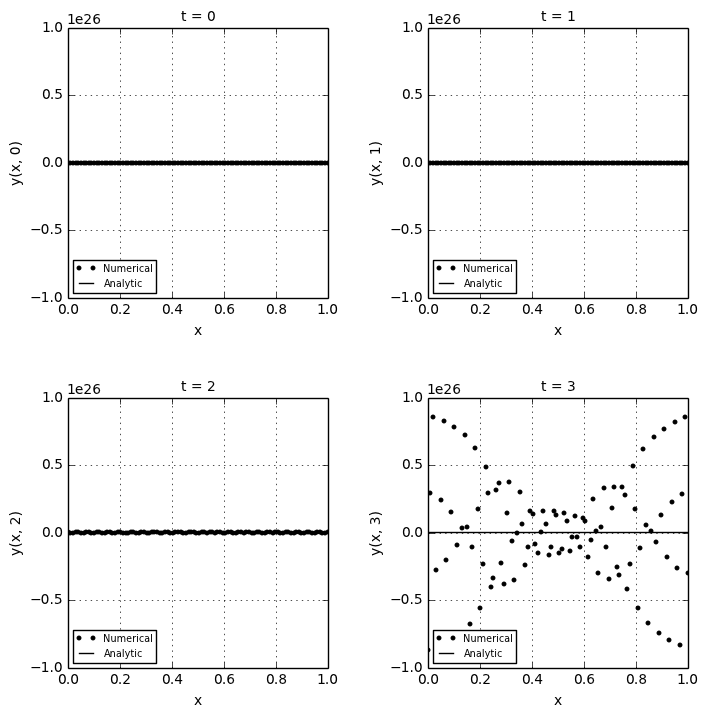
\includegraphics[width=1\columnwidth, resolution=600, resolution=600]{q1_ftcs.pdf} 

        \caption{\label{fig:ftcs} Snapshots of $y$ at different times as a
        function of $x$ using the FTCS scheme. The FTCS scheme reproduces the
        analytic results Equation~\ref{eq:y} terribly. The numerical
        progression of $y(x,t)$ diverged.}

    \end{center}
    \end{figure}
    %---------------------------------------------------------------------------

\end{homeworkProblem}
\clearpage
%===============================================================================


%===============================================================================
%-------------------------------------------------------------------------------
%	PROBLEM 2 
%-------------------------------------------------------------------------------
\begin{homeworkProblem}

    The Forward-Time Forward-Space (FTFS) scheme can be calculated numerically
    by 

    \begin{equation}
        y^{n+1}_k = y^n_k - a(t^{n+1} - t^n)  \
        \frac{y^n_{k+1} - y^n_k}{x_{k+1} - x_k}
    \end{equation}

    \noindent and the Forward-Time Backward-Space (FTFS) scheme can be
    calculated numerically by 

    \begin{equation}
        y^{n+1}_k = y^n_k - a(t^{n+1} - t^n)  \
        \frac{y^n_{k} - y^n_{k-1}}{x_{k} - x_{k-1}}
    \end{equation}

    We ran the numerical simulation of the progression of $y(x,t)$ using the
    same parameters and boundaries as in Problem 1.  Figures~\ref{fig:q2_ftfs}
    and~\ref{fig:q2_ftbs} show the results of the simulations.

    %---------------------------------------------------------------------------
    % FIGURE
    \begin{figure}[!ht]
    \begin{center}
        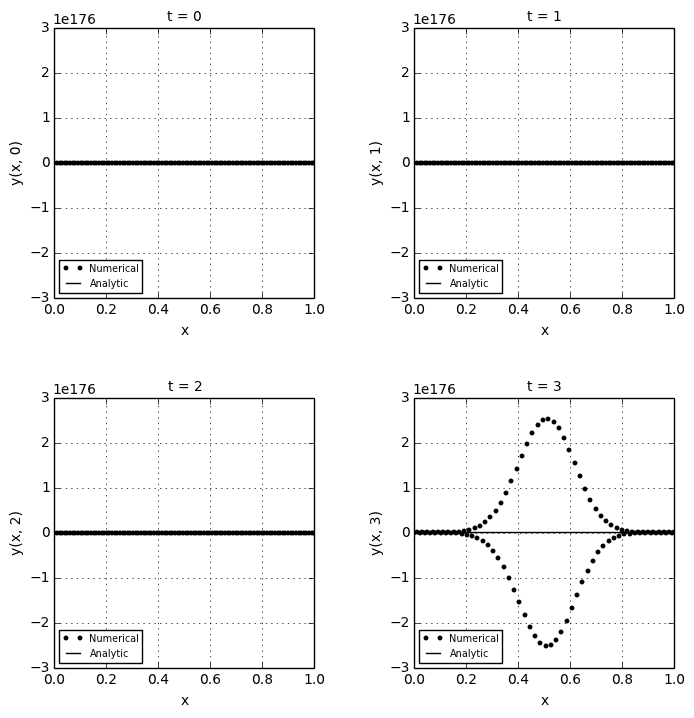
\includegraphics[width=1\columnwidth, resolution=600]{q2_ftfs.pdf} % Example image

        \caption{\label{fig:q2_ftfs} Snapshots of $y$ at different times as a
        function of $x$ using the FTFS scheme. The FTFS scheme reproduces the
        analytic results Equation~\ref{eq:y} terribly given the parameters in
        Problem 1. The numerical progression of $y(x,t)$
        diverged.}

    \end{center}
    \end{figure}
    %---------------------------------------------------------------------------
    
    %---------------------------------------------------------------------------
    % FIGURE
    \begin{figure}[!ht]
    \begin{center}
        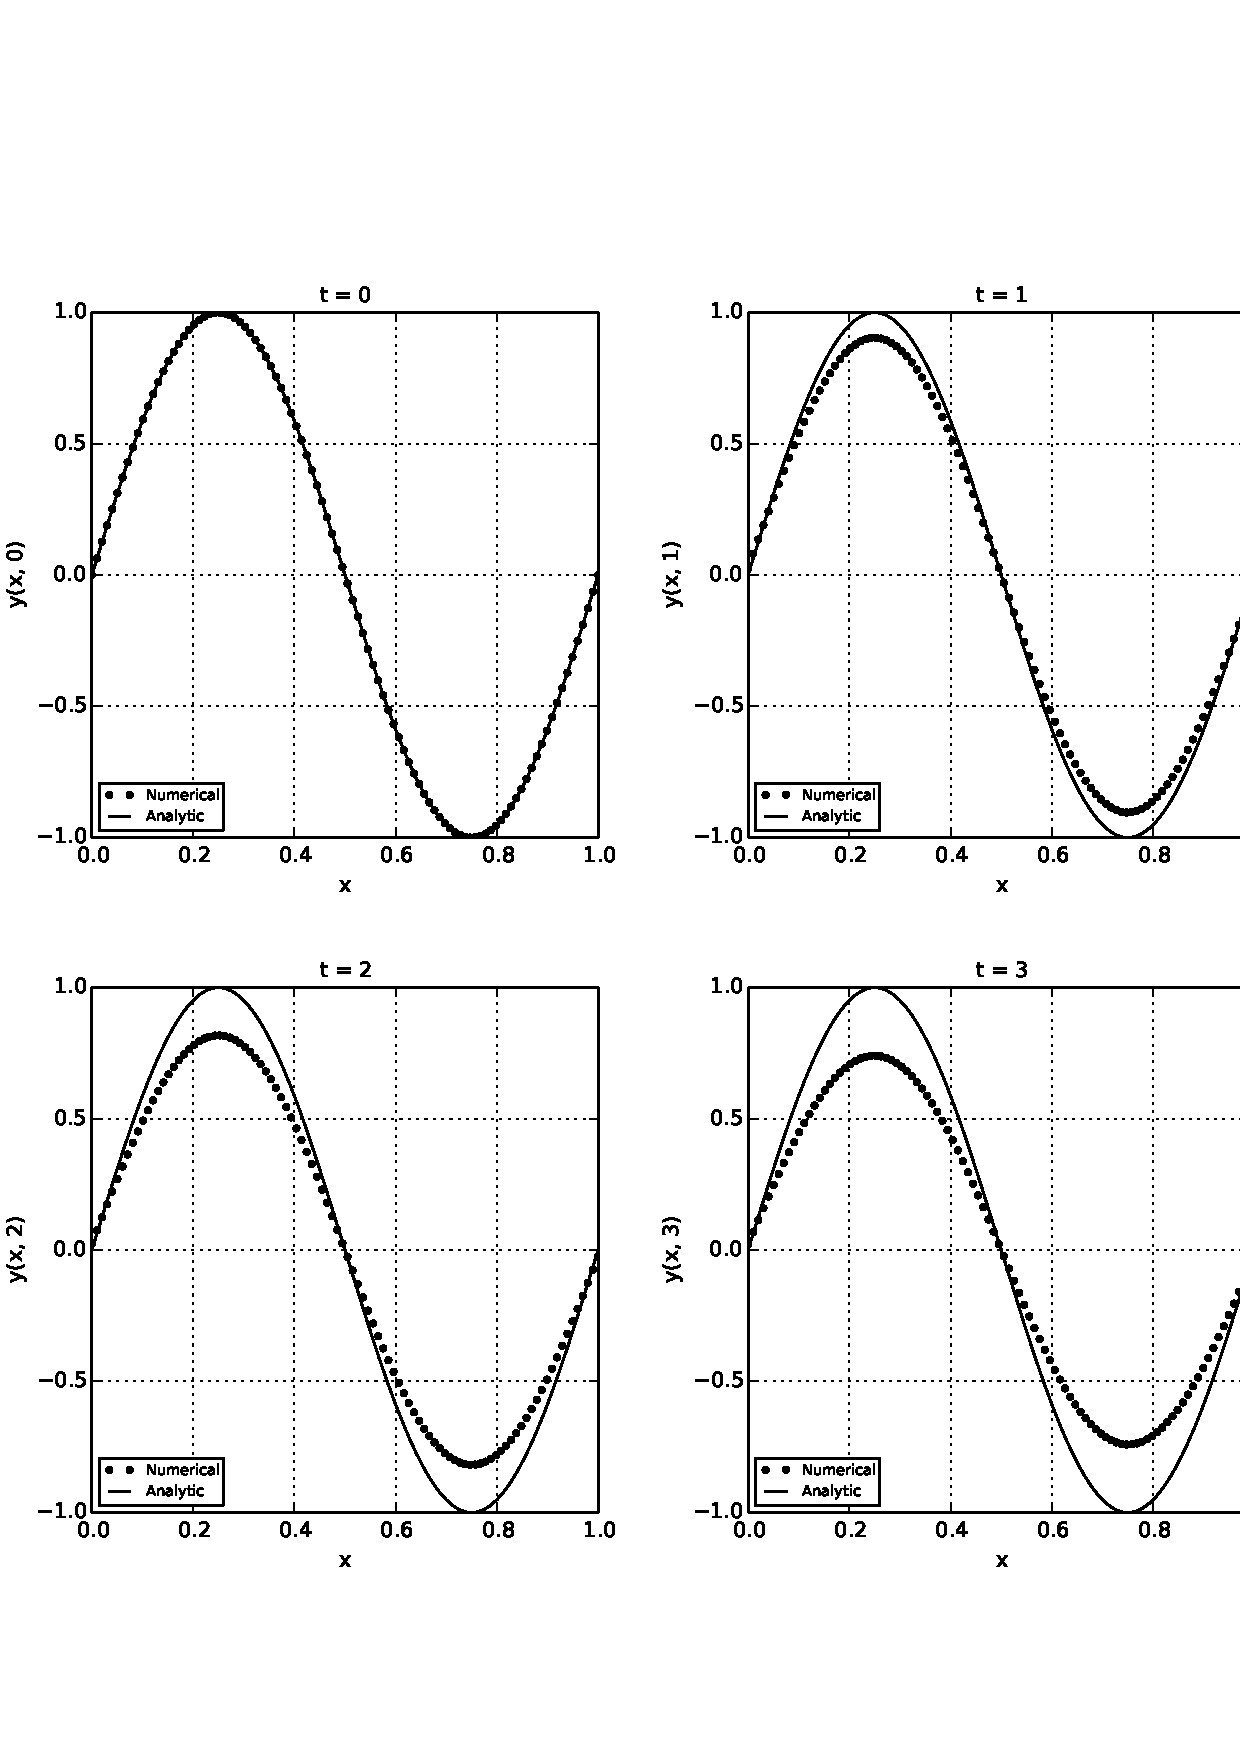
\includegraphics[width=1\columnwidth, resolution=600]{q2_ftbs.pdf} % Example image

        \caption{\label{fig:q2_ftbs}Snapshots of $y$ at different times as a
        function of $x$ using the FTBS scheme. The FTBS scheme reproduces the
        analytic results Equation~\ref{eq:y} mildly well given the parameters
        in Problem 1. The numerical progression of $y(x,t)$ is decreasing in
        amplitude from the analytic result with time. This is an example of
        numerical diffusion.}

    \end{center}
    \end{figure}
    %---------------------------------------------------------------------------


\end{homeworkProblem}
\clearpage
%===============================================================================

%===============================================================================
%-------------------------------------------------------------------------------
%	PROBLEM 3
%-------------------------------------------------------------------------------
\begin{homeworkProblem}

    We ran the numerical simulation of the progression of $y(x,t)$ using the
    same parameters and boundaries as in Problem 1 except we set the flow
    speed, $a = -1$.  Figures~\ref{fig:q3_ftfs} and~\ref{fig:q3_ftbs} show the
    results of the simulations.

    %---------------------------------------------------------------------------
    % FIGURE
    \begin{figure}[!ht]
    \begin{center}
        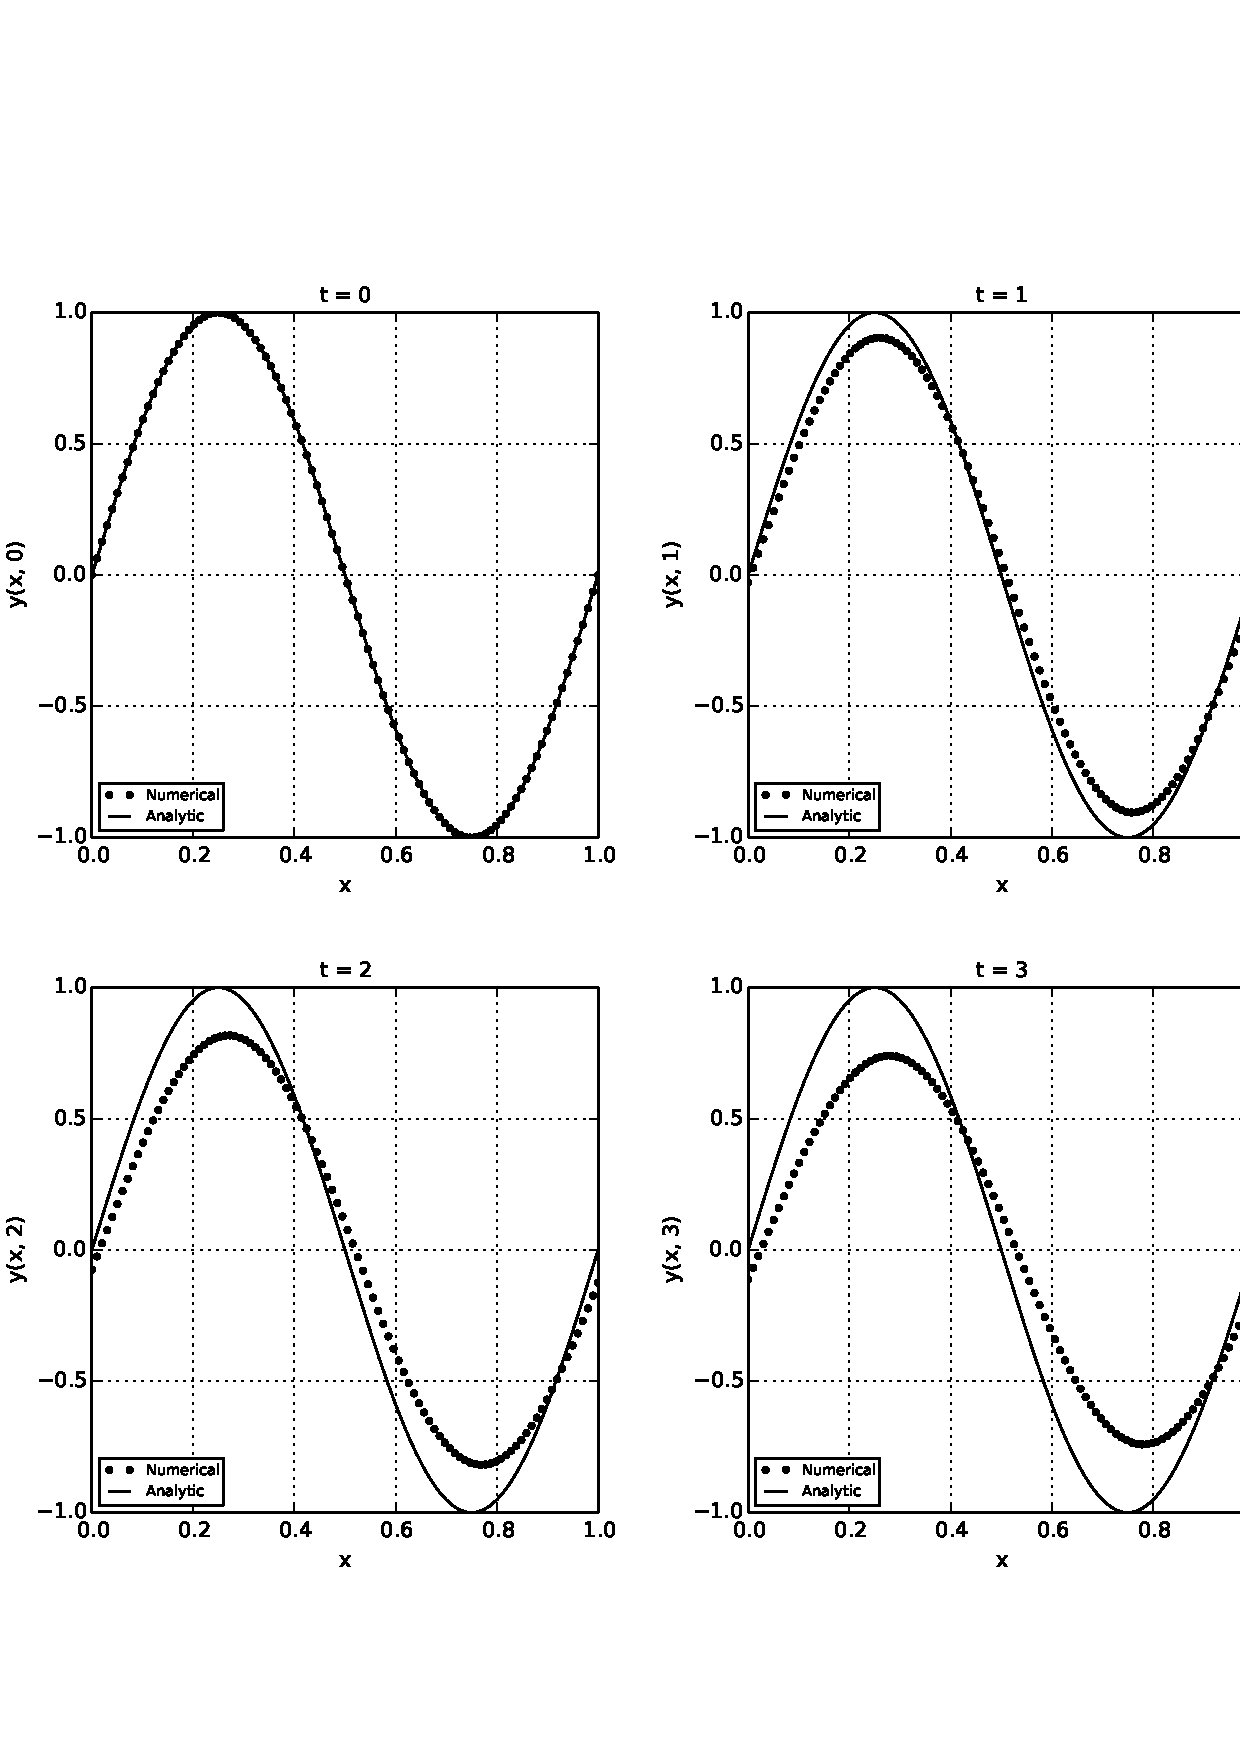
\includegraphics[width=1\columnwidth, resolution=600]{q3_ftfs.pdf} % Example image

        \caption{\label{fig:q3_ftfs} Snapshots of $y$ at different times as a
        function of $x$ using the FTFS scheme. The FTFS scheme reproduces the
        analytic results Equation~\ref{eq:y} mildly well given the parameters in
        Problem 1. The numerical progression of $y(x,t)$ is decreasing in
        amplitude from the analytic result with time. Because the flow speed
        switched directions the FTFS scheme is now calculating the progression
        of $y$ from upstream instead of downstream.}

    \end{center}
    \end{figure}
    %---------------------------------------------------------------------------
    
    %---------------------------------------------------------------------------
    % FIGURE
    \begin{figure}[!ht]
    \begin{center}
        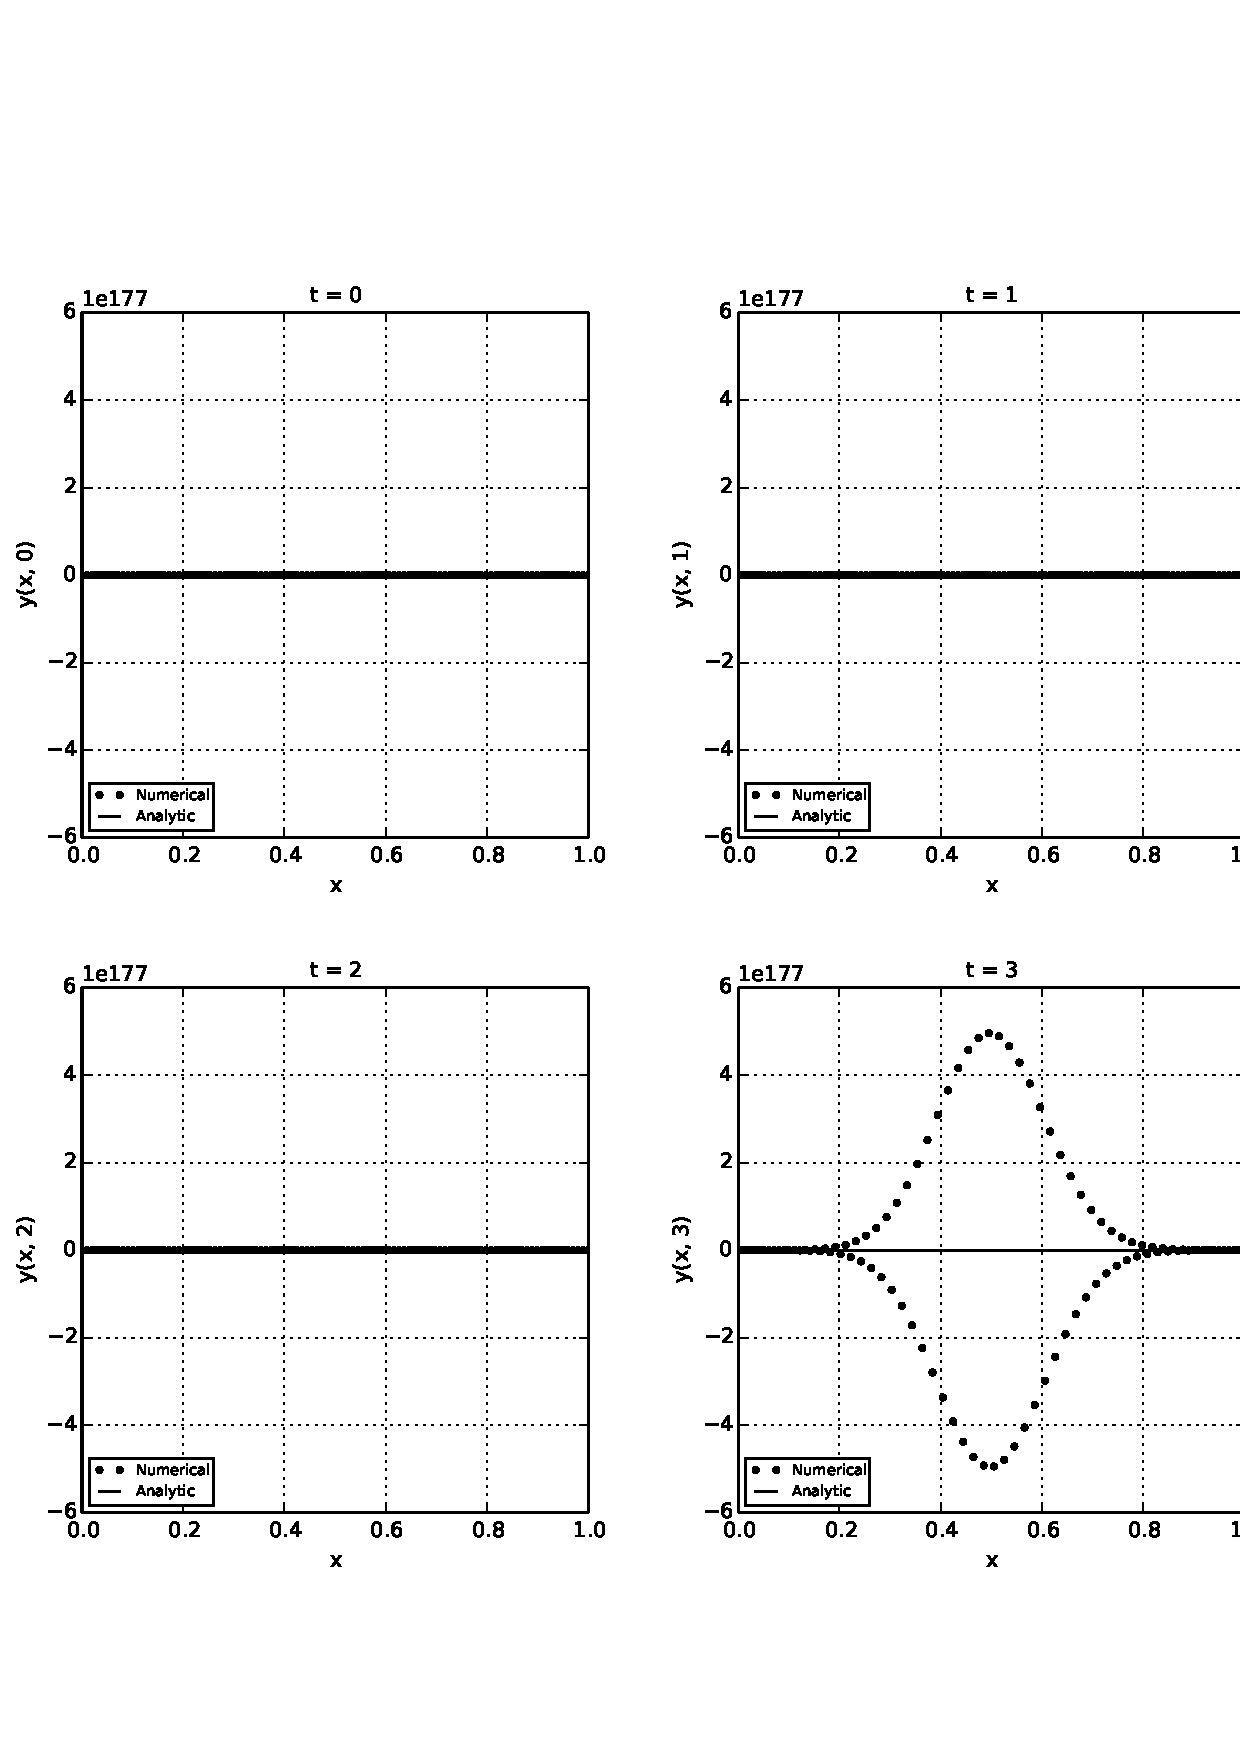
\includegraphics[width=1\columnwidth, resolution=600]{q3_ftbs.pdf} % Example image

        \caption{\label{fig:q3_ftbs}Snapshots of $y$ at different times as a
        function of $x$ using the FTBS scheme. The FTBS scheme reproduces the
        analytic results Equation~\ref{eq:y} terribly given the parameters in
        Problem 1. The numerical progression of $y(x,t)$ diverged. Because the
        flow speed switched directions the FTBS scheme is now calculating the
        progression of $y$ from downstream instead of upstream.}

    \end{center}
    \end{figure}
    %---------------------------------------------------------------------------



\end{homeworkProblem}
\clearpage
%===============================================================================

%===============================================================================
%-------------------------------------------------------------------------------
%	PROBLEM 4
%-------------------------------------------------------------------------------
\begin{homeworkProblem}

    To apply a von Neumann stability analysis on the Forward-Time Forward-Space
    (FTFS) scheme: since $x_k = k \Delta x$, the initial state at $t = 0$ can
    be written as

    \begin{equation}
        y_k^0 = \sin[2 \pi k \Delta x]
    \end{equation}

    \noindent which we then substitute into the FTFS scheme

    \begin{equation}
        y^{n+1}_k = y^n_k + a(t^{n+1} - t^n)  \
        \frac{y^n_{k+1} - y^n_k}{x_{k+1} - x_k}
    \end{equation}

    \noindent to get the solution after a single time-step

    \begin{equation}
        y_k^1 = \sin[2 \pi k \Delta x] - a \Delta t 
        \frac{\sin[2 \pi (k+1) \Delta x] - \sin[2 \pi k \Delta x]}{\Delta x}
    \end{equation}

    Setting $a \Delta t / \Delta x = \alpha$ we get

    \begin{equation}
        y_k^1 = \sin[2 \pi k \Delta x] -
        \alpha \sin[2 \pi k \Delta x + 2 \pi \Delta x ] - \sin[2 \pi k \Delta x]
    \end{equation}

    \noindent using the identity

    \begin{equation}
        \sin[\theta] \pm \sin[\phi] = 
        2 \sin[\frac{\theta \pm \phi}{2}] \cos[\frac{\theta \mp \phi}{2}]
    \end{equation}

    \begin{equation}
        y_k^1 = \sin[2 \pi k \Delta x] - 2 \alpha
        \sin[\frac{2 \pi k \Delta x + 2 \pi \Delta x - 2 \pi k \Delta x}{2}] 
        \cos[\frac{2 \pi k \Delta x+ 2 \pi \Delta x + 2 \pi k \Delta x}{2}]
    \end{equation}

    \begin{equation}
        y_k^1 = \sin[2 \pi k \Delta x] - 2 \alpha
        \sin[\pi \Delta x] 
        \cos[2 \pi k \Delta x + \pi \Delta x ]
    \end{equation}

    \noindent using the identity

    \begin{equation}
        \cos[\theta \pm \phi] = 
        \cos[\theta] \cos[\phi] \mp \sin[\theta] \sin[\phi]
    \end{equation}

    \begin{equation}
        y_k^1 = \sin[2 \pi k \Delta x] - 2 \alpha
        \sin[\pi \Delta x] 
        [\cos[2 \pi k \Delta x] \cos[ \pi \Delta x ] - 
            \sin[2 \pi k \Delta x] \sin[ \pi \Delta x ]]
    \end{equation}

    \begin{equation}
        y_k^1 = \sin[2 \pi k \Delta x] - 2 \alpha
        \sin[\pi \Delta x] 
        [\cos[ \pi \Delta x ] \sin[ \pi \Delta x ] \cos[2 \pi k \Delta x]  - 
            \sin^2[\pi \Delta x] \sin[ 2 \pi k \Delta x ]]
    \end{equation}

    \begin{equation}
        y_k^1 = (1 + 2 \alpha \sin^2[\pi \Delta x] )\sin[2 \pi k \Delta x] 
        + 2 \alpha \cos[ \pi \Delta x ] \sin[ \pi \Delta x ] 
        \cos[2 \pi k \Delta x]      
    \end{equation}

    \noindent using the identities

    \begin{equation}
        \sin^2[\theta] = \frac{1 - \cos[2\theta]}{2}
        \,\,\,\,\,\,\,\,\,\,\,\,
        \cos[\theta] \sin[\theta] = 
        \frac{\sin[2 \theta]}{2}
    \end{equation}

    \begin{equation}
        y_k^1 = (1 - \frac{2 \alpha}{2} (1 - \cos[2 \pi \Delta x])) 
            \sin[2 \pi k \Delta x] 
            + \frac{2 \alpha}{2} \sin[2 \pi \Delta x ]
            \cos[2 \pi k \Delta x]      
    \end{equation}

    We define the grid parameter $G \equiv 1 - \cos[2 \pi \Delta x]$ thus
    
    \begin{equation} \label{eq:G}
        y_k^1 = (1 - G \alpha )\sin[2 \pi k \Delta x] 
            + \alpha \sin[2 \pi \Delta x ]
            \cos[2 \pi k \Delta x]      
    \end{equation}

    \noindent using the identity

    \begin{equation}
        a \sin[\theta] + b\cos[\theta] = c \sin[\theta - \phi]
    \end{equation}

    \noindent where $c = \sqrt{a^2 + b^2}$ and $\phi = {\rm atan2}[b,a]$, we
    can arrange Eq.~\ref{eq:G} to be

    \begin{equation}
        y_k^1 = A \sin[2 \pi \Delta x + \phi]
    \end{equation}

    \noindent where

    \begin{equation}
        A = \sqrt{{(1 + G\alpha)}^2 + \alpha^2 \sin^2[2 \pi \Delta x]}
        \,\,\,\,\,\,\,\,\,\,\,\,
        \phi = {\rm atan2}[- \alpha \sin[2 \pi \Delta x ], 1+G \alpha] 
    \end{equation}

    We can manipulate $G^2$ by setting $\theta = 2 \pi \Delta x$ and then

    \begin{align*}
        G \equiv &\ 1 - \cos[\theta] \\
        G^2 = &\ 1 - 2 \cos[\theta] + \cos^2[\theta]  \\
        G^2 = &\ 1 - 2 \cos[\theta] + 1 - \sin^2[\theta]  \\
        G^2 = &\ 2 - 2 (1 - G) - \sin^2[\theta]
    \end{align*}

    \noindent thus

    \begin{equation}\label{eq:sin2g}
        \sin^2[\theta] = 2G - G^2 
    \end{equation}

    \noindent which we can substitute into A, to get 
    
    \begin{equation}
        A = \sqrt{{(1+G\alpha)}^2 + \alpha^2(2G-G^2)}
    \end{equation}
    
    \begin{equation}
        A = \sqrt{{(1+2G\alpha+G^2\alpha^2)} + 2\alpha^2G-\alpha^2G^2}
    \end{equation}
    
    \begin{equation}
        A = \sqrt{1+2G\alpha(\alpha+1)}
    \end{equation}

    %---------------------------------------------------------------------------
    % Answer

    \problemAnswer{Finally, for any given number of time s.pdf, $n$, using the
    Forward-Time Forward-Space scheme we will have

    \begin{equation}
        y_k^n = A^n \sin[2 \pi \Delta x + n \phi]
    \end{equation}
    
    \noindent where

    \begin{equation}\label{eq:amp_ftfs}
        A = \sqrt{1+2G\alpha(\alpha+1)}
        \,\,\,\,\,\,\,\,\,\,\,\,
        \phi = {\rm atan2}[-\alpha \sin[2 \pi \Delta x ], (1 + G \alpha)] 
    \end{equation}}
    %---------------------------------------------------------------------------
    
    \vspace{1cm}

    To apply a von Neumann stability analysis on the Forward-Time Backward-Space
    (FTBS) scheme: since $x_k = k \Delta x$, the initial state at $t = 0$ can
    be written as

    \begin{equation}
        y^{n+1}_k = y^n_k - a(t^{n+1} - t^n)  \
        \frac{y^n_{k} - y^n_{k-1}}{x_{k} - x_{k-1}}
    \end{equation}

    \noindent to get the solution after a single time-step

    \begin{equation}
        y_k^1 = \sin[2 \pi k \Delta x] + a \Delta t 
        \frac{\sin[2 \pi k \Delta x] - \sin[2 \pi (k-1) \Delta x]}{\Delta x}
    \end{equation}

    Following the same methods as for the FTFS stability analysis, we reveal
    the progression of amplitudes as a function of time and space:

    %---------------------------------------------------------------------------
    % Answer

    \problemAnswer{For any given number of time s.pdf, $n$, using the
    Forward-Time Backward-Space scheme we will have

    \begin{equation}
        y_k^n = A^n \sin[2 \pi \Delta x + n \phi]
    \end{equation}
    
    \noindent where

    \begin{equation}\label{eq:amp_ftbs}
        A = \sqrt{1+2G\alpha(\alpha-1)}
        \,\,\,\,\,\,\,\,\,\,\,\,
        \phi = {\rm atan2}[\alpha \sin[2 \pi \Delta x ], (1 - G \alpha)] 
    \end{equation}}
    %---------------------------------------------------------------------------
    \vspace{1cm} 


\end{homeworkProblem}
%===============================================================================


%===============================================================================
%-------------------------------------------------------------------------------
%	PROBLEM 5 
%-------------------------------------------------------------------------------
\begin{homeworkProblem}
    
    Figure~\ref{fig:stability} analyzes the stability of FTFS and FTBS schemes
    across a range of $G$ and $\alpha$. 

    %---------------------------------------------------------------------------
    % FIGURE
    \begin{figure}[!ht]
    \begin{center}
        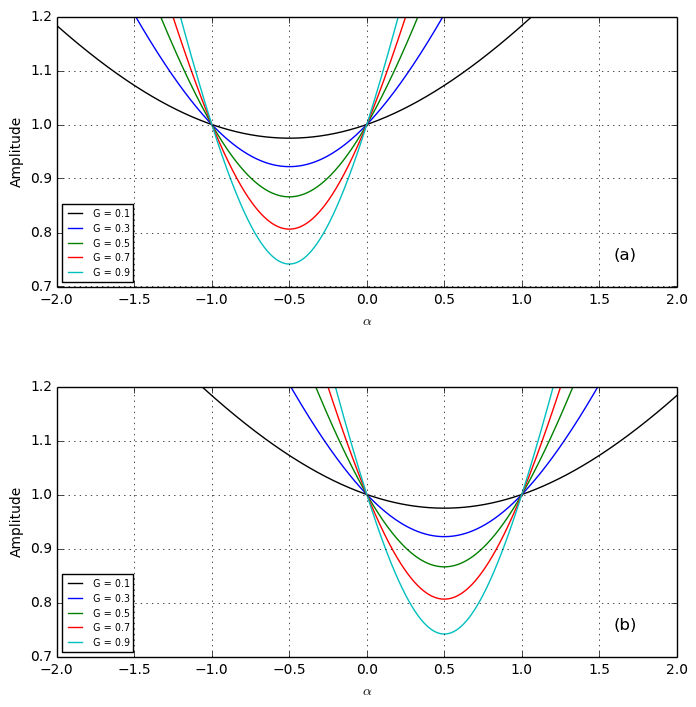
\includegraphics[width=1\columnwidth, resolution=600]{q5.pdf} % Example image

        \caption{\label{fig:stability} Amplitudes of (a): FTFS scheme and (b):
        FTBS scheme as a function of $\alpha$ for different $G$ values (see
        Equations~\ref{eq:amp_ftfs} and~\ref{eq:amp_ftbs} respectively). The
        amplitude of the flow will remain finite as a function of time in the
        FTFS scheme for $0 < \alpha < 1$, and for the FTBS scheme for $-1 <
        \alpha < 0$. This means that only upstream schemes will provide stable
        progressions of flow amplitudes for $|\alpha| < 1$.}

    \end{center}
    \end{figure}
    %---------------------------------------------------------------------------

\end{homeworkProblem}
\clearpage
%===============================================================================

%===============================================================================
%-------------------------------------------------------------------------------
%	PROBLEM 6
%-------------------------------------------------------------------------------
\begin{homeworkProblem}

    Figure~\ref{fig:q6_ftbs} demonstrates the result of running a upstream
    scheme with $|\alpha| > 1$. The numerical progression of $y(x,t)$ diverged.
    $\alpha$ is now $> 2$ hence the amplitude will diverge from solution
    because the FTBS scheme is calculating the progression of $y$ from
    downstream instead of upstream.

    %---------------------------------------------------------------------------
    % FIGURE
    \begin{figure}[!ht]
    \begin{center}
        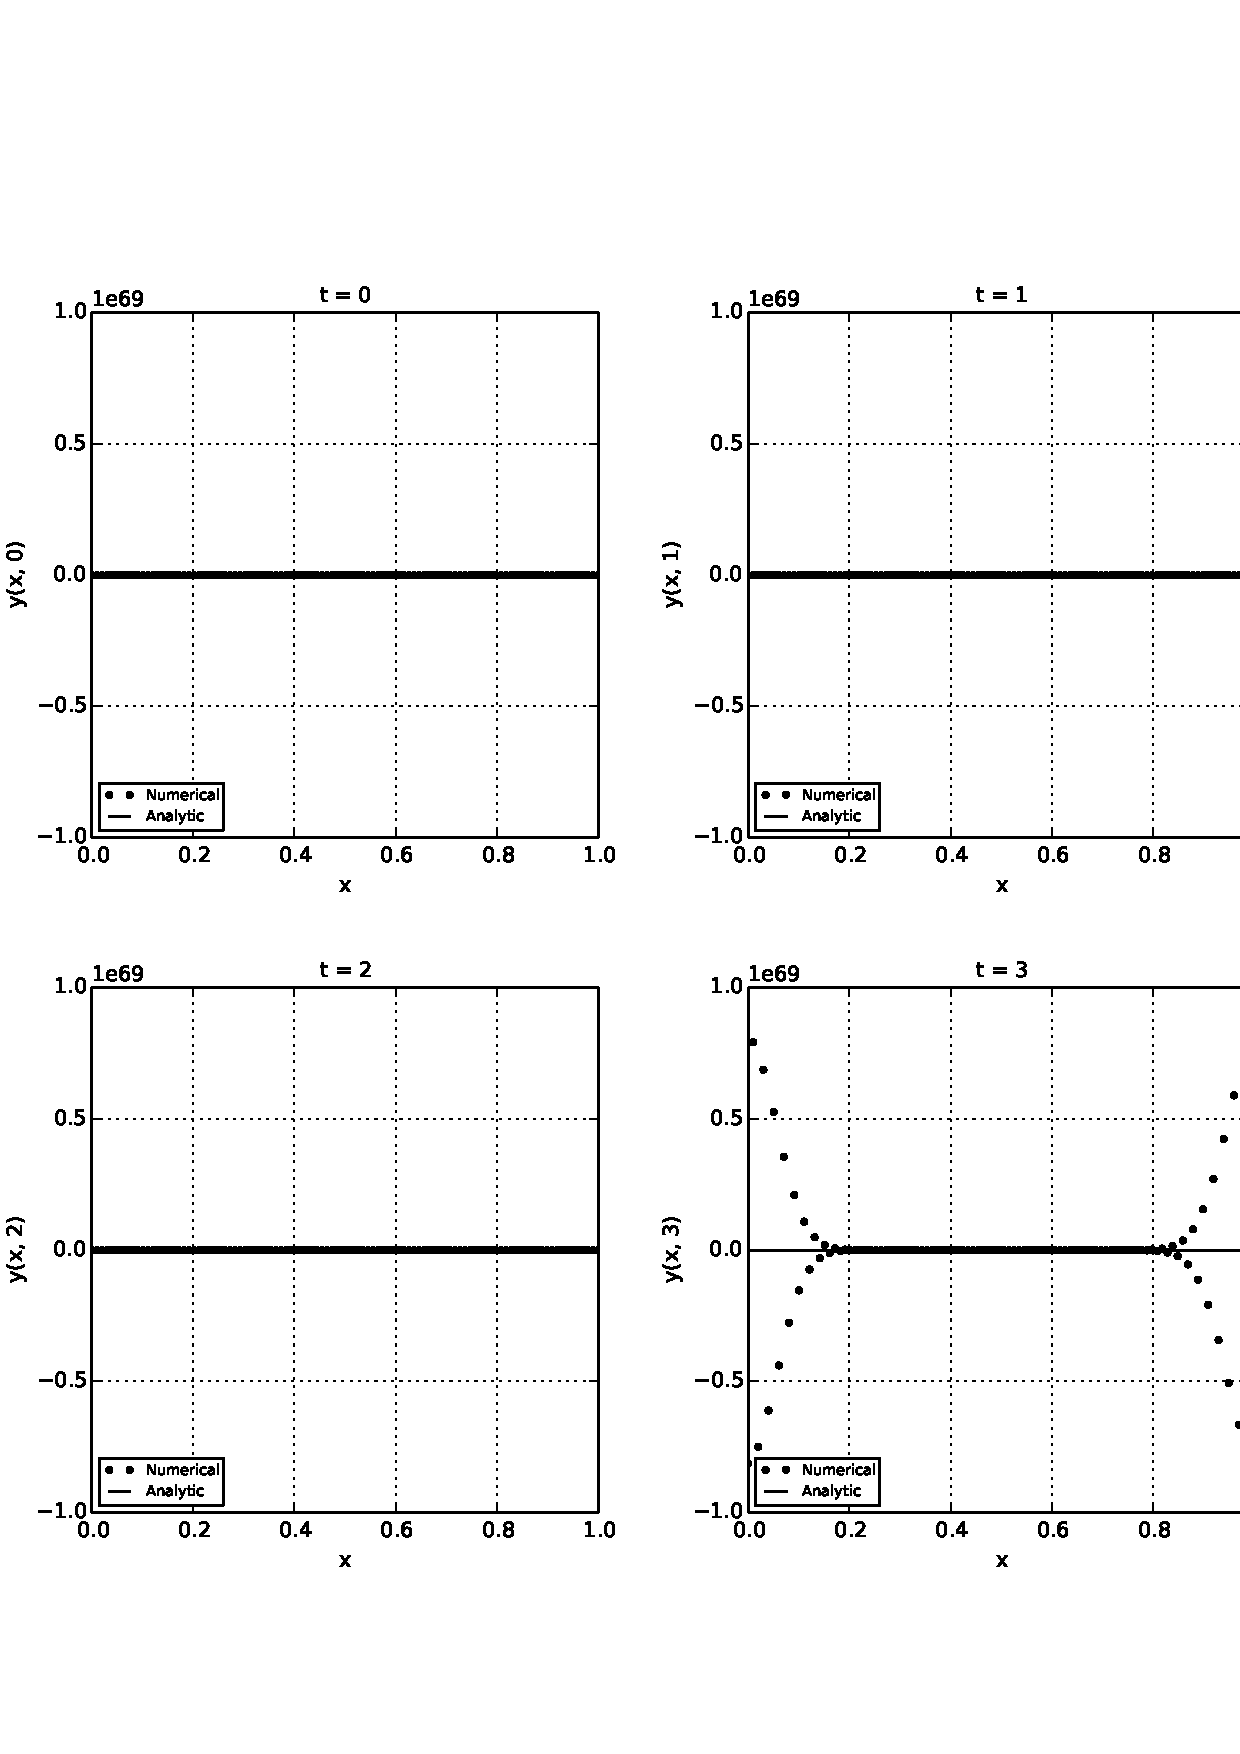
\includegraphics[width=1\columnwidth, resolution=600]{q6_ftbs.pdf} % Example image

        \caption{\label{fig:q6_ftbs} Snapshots of $y$ at different times as a
        function of $x$ using the FTBS scheme. The FTBS scheme reproduces the
        analytic results Equation~\ref{eq:y} terribly given a flow speed of 1
        and $\alpha = 2$. The numerical progression of $y(x,t)$ diverged.
        Because $\alpha$ is now $> 2$ the amplitude will diverge from solution.
        The FTBS scheme is calculating the progression of $y$ from downstream
        instead of upstream.}

    \end{center}
    \end{figure}
    %---------------------------------------------------------------------------

\end{homeworkProblem}
\clearpage
%===============================================================================

%===============================================================================
%-------------------------------------------------------------------------------
%	PROBLEM 7
%-------------------------------------------------------------------------------
\begin{homeworkProblem}

    Figure~\ref{fig:p7} demonstrates the affect of choosing different $\alpha$
    values in a stable scheme. The numerical diffusion is greater for $\alpha =
    0.25$ than for $\alpha = 0.5$ because the simulation with $\alpha = 0.25$
    needs more time s.pdf to reach the same time as for the $\alpha = 0.5$
    simulation, despite the diffusion amplitude being closer to 1 for $\alpha =
    0.25$.

    %---------------------------------------------------------------------------
    % FIGURE
    \begin{figure}[!ht]
    \begin{center}
        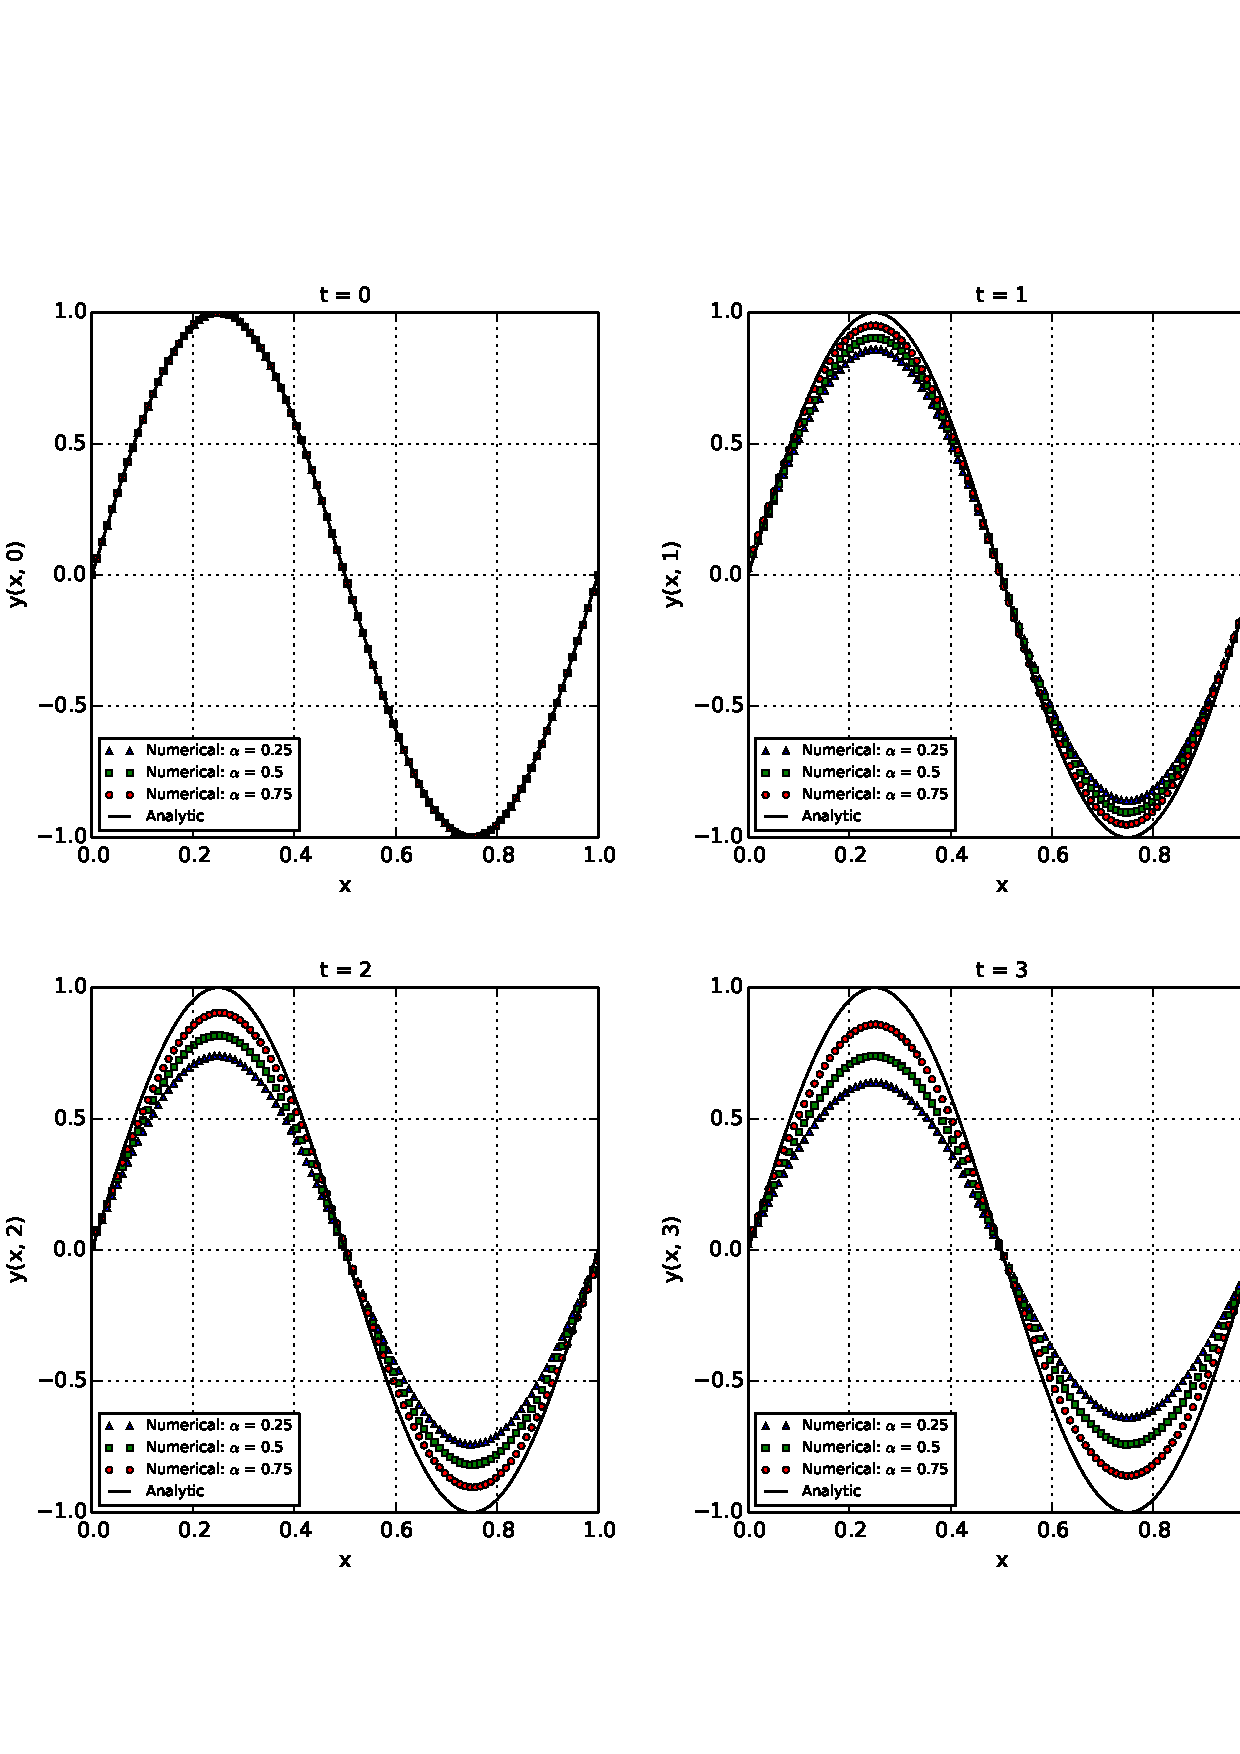
\includegraphics[width=1\columnwidth, resolution=600]{q7.pdf} % Example image

        \caption{\label{fig:p7} Snapshots of $y$ at different times as a
        function of $x$ using the FTBS scheme given a flow speed of 1 and
        and with varying $\alpha$ values.}

    \end{center}
    \end{figure}
    %---------------------------------------------------------------------------

\end{homeworkProblem}
\clearpage
%===============================================================================

%===============================================================================
%-------------------------------------------------------------------------------
%	PROBLEM 8
%-------------------------------------------------------------------------------
\begin{homeworkProblem}

    Our BTCS scheme was derived beginning with

    \begin{equation}
        y^{n+1}_k = y^n_k + a(t^{n+1} - t^n)  \
        \frac{y^n_{k+1} - y^n_k}{x_{k+1} - x_k}
    \end{equation}

    \noindent and next solving for $y^n_k$

    \begin{equation}
        y^{n}_k = y^{n+1}_k - \alpha y^{n+1}_{k+1} + \alpha y^{n+1}_{k-1} 
    \end{equation}

    \noindent whereby we can construct a $K \times K$ matrix $M$ to solve the
    scheme for forward times

    \begin{equation}
        M =
         \begin{pmatrix}
          1 & -\alpha & \cdots & \alpha \\
          \alpha & 1 & \cdots & 0 \\
          \vdots  & \vdots  & \ddots & \vdots  \\
          -\alpha & \alpha & \cdots & 1
         \end{pmatrix}
    \end{equation}

    \begin{equation}
        M 
        \begin{pmatrix}
            y^{n+1}_{0} \\
            y^{n+1}_{1} \\
            \vdots \\
            y^{n+1}_{K-1} \\
        \end{pmatrix}
        =
        \begin{pmatrix}
            y^{n}_{0} \\
            y^{n}_{1} \\
            \vdots \\
            y^{n}_{K-1} \\
        \end{pmatrix}
    \end{equation}

    \noindent which allows us to solve for future time s.pdf from an initial
    condition.\\

    Figure~\ref{fig:p8} shows simulation results from the backward-time
    centered-space (BTCS) scheme. \\
    
    %---------------------------------------------------------------------------
    % FIGURE
    \begin{figure}[!ht]
    \begin{center}
        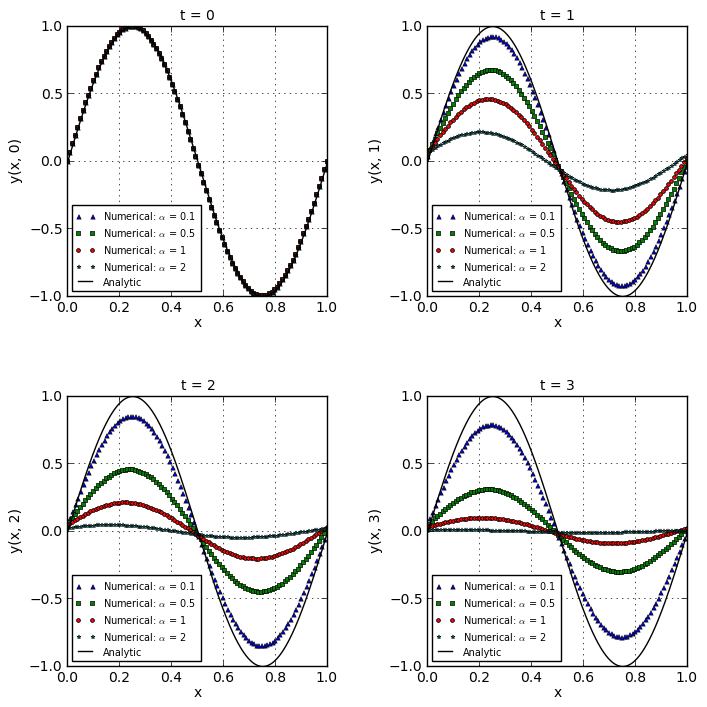
\includegraphics[width=1\columnwidth, resolution=600, resolution=600]{q8.pdf} 

        \caption{\label{fig:p8} Snapshots of $y$ at different times as a
        function of $x$ using the BTCS scheme given a flow speed of 1 and
        and with varying $\alpha$ values. The BTCS scheme is much more stable
        than the FTBS or FTFS schemes for any choice of $\alpha$, though
        numerical diffusion may be prominent.}

    \end{center}
    \end{figure}
    %---------------------------------------------------------------------------
    \clearpage

    To apply a von Neumann stability analysis on the BTCS scheme we substitute
    the initial the initial state at $t = 0$ 

    \begin{equation}
        y_k^0 = \sin[2 \pi k \Delta x]
    \end{equation}

    \noindent which we then substitute into the BTCS scheme

    \begin{equation}
        y^{n-1}_k = y^{n}_k + a(t^{n} - t^n)  \
        \frac{y^{n}_{k+1} - y^{n}_{k-1}}{x_{k+1} - x_{k-1}} =
        y^{n}_k + \frac{a\Delta t}{2 \Delta x}  \
        (y^{n}_{k+1} - y^{n}_{k-1})
    \end{equation}

    \noindent to get the solution before a single time-step we assumed an
    ansatz of 

    \begin{equation}
        y^n_k = A^n e^{ki2\pi\Delta x}
    \end{equation}

    \noindent and substituted this into the BTCS scheme to get

    \begin{equation}
        A^{n-1} e^{ki2\pi \Delta x} = 
        A^{n} e^{ki2\pi \Delta x} +
        \frac{\alpha}{2}[A^{n} e^{(k+1)i2\pi \Delta x} +
        A^{n} e^{(k-1)i2\pi \Delta x}]
    \end{equation}

    \begin{equation}
        A^{n} A^{-1} e^{ki2\pi \Delta x} = 
        A^{n} e^{ki2\pi \Delta x} 
        [1 + \frac{\alpha}{2}[e^{2\pi \Delta x} + e^{-2\pi \Delta x}]]
    \end{equation}

    \noindent leading to a solution for the amplification factor $A$

    \begin{equation}
        A = \frac{1}{1+\frac{\alpha}{2}[e^{2\pi \Delta x} - e^{-2\pi \Delta x}]}
    \end{equation}

    \begin{equation}
        A = \frac{1}{1+\frac{\alpha}{2}2i \sin[2\pi \Delta x]}
    \end{equation}

    \noindent whose modulus is

    \begin{equation}
        A = \frac{1}{\sqrt{1+\alpha^2 \sin^2[2\pi \Delta x]}}
    \end{equation}
    
    \noindent in which we substitute Equation~\ref{eq:sin2g} to get

    \begin{equation}
        A = \frac{1}{\sqrt{1+\alpha^2(2G-G^2)}}
    \end{equation}


    %---------------------------------------------------------------------------
    % Answer

    \problemAnswer{Finally, for any given number of time s.pdf, $n$, using the
    Backward-Time Center-Space scheme we will have

    \begin{equation}
        y_k^{n} = A^{n} e^{ki2\pi \Delta x} 
    \end{equation}
    
    \noindent where

    \begin{equation}\label{eq:amp_btcs}
        A = \frac{1}{\sqrt{1+\alpha^2(2G-G^2)}}
    \end{equation}

    For any choice of $\alpha$ and $G$, $A < 1$. Figure~\ref{fig:p8_amp}
    demonstrates this result for the BTCS scheme.}
    %---------------------------------------------------------------------------
    
    %---------------------------------------------------------------------------
    % FIGURE
    \begin{figure}[!ht] 
    \begin{center} 
        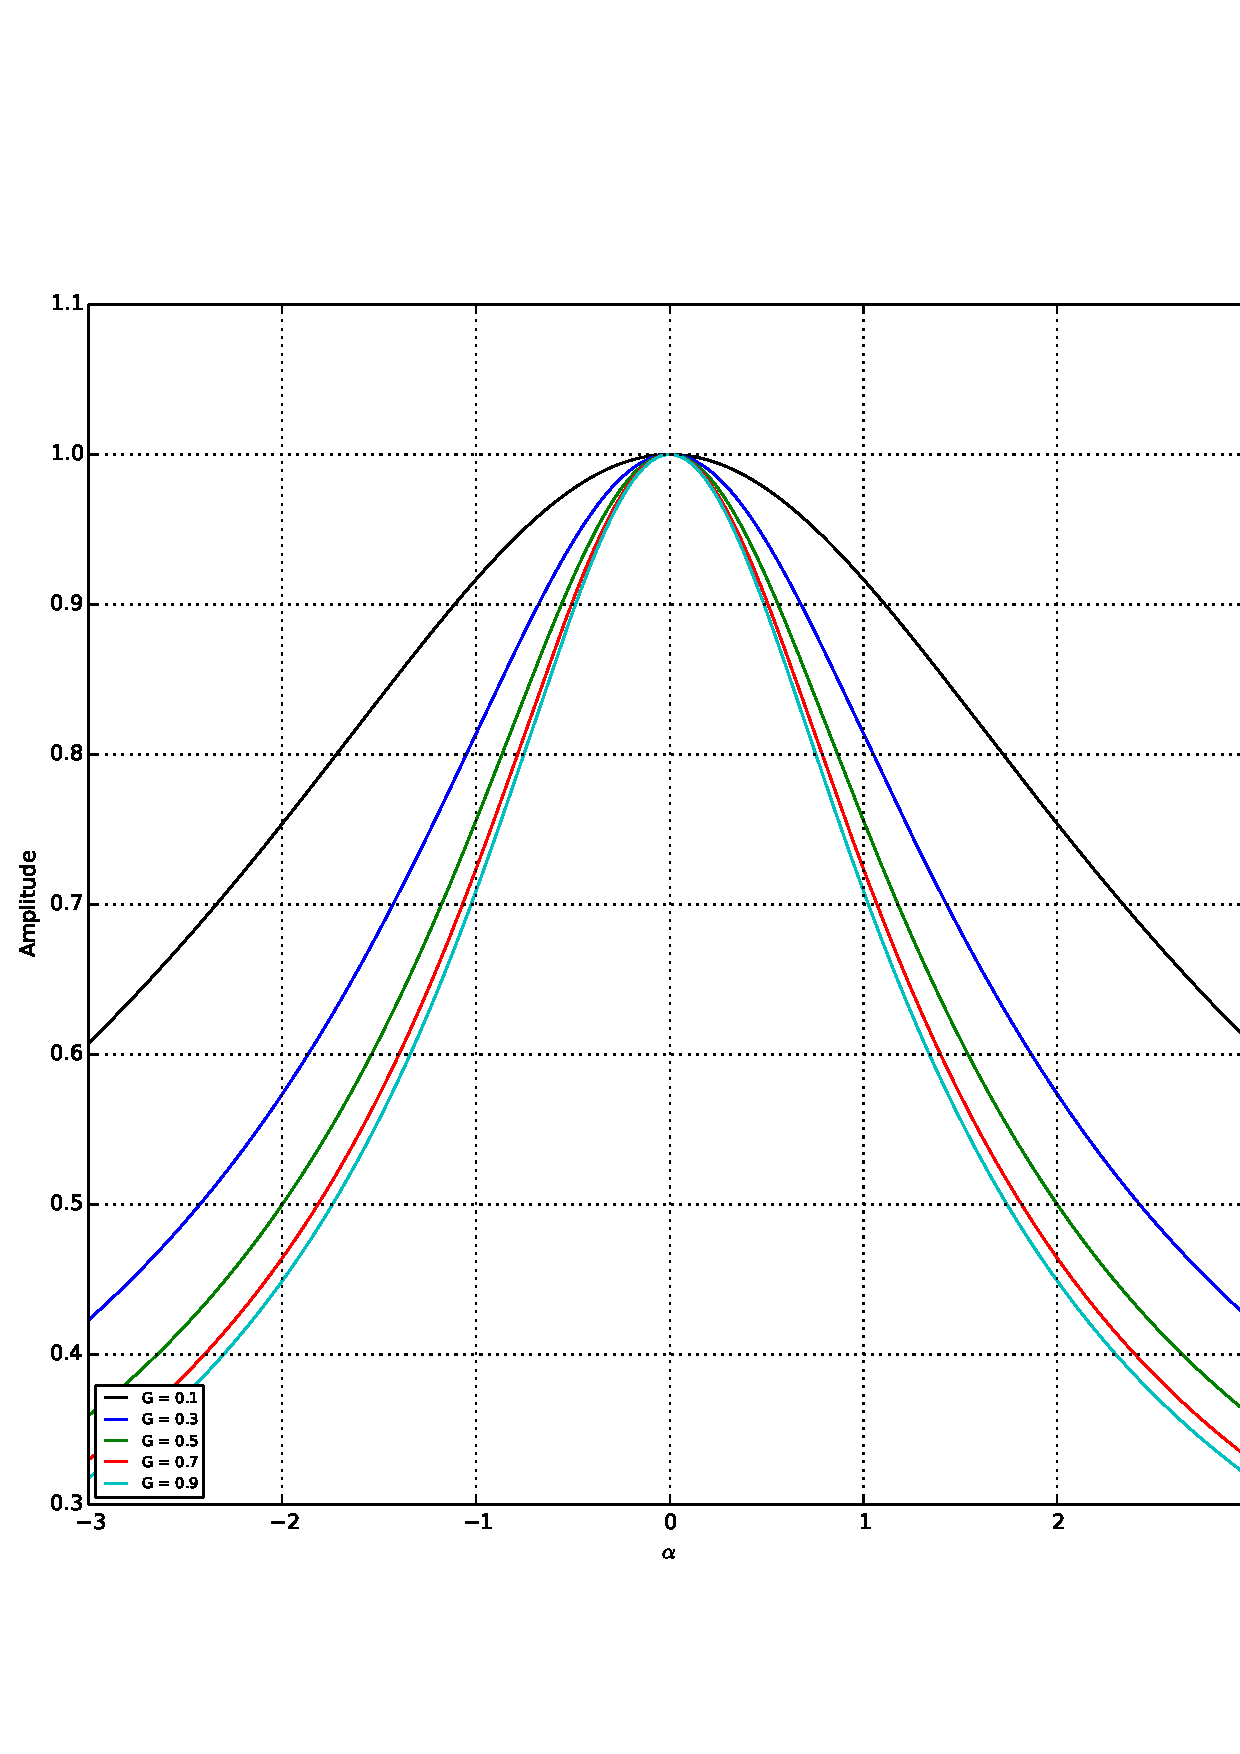
\includegraphics[width=1\columnwidth, resolution=600]{q8_amp.pdf} % Example image

        \caption{\label{fig:p8_amp} Amplitudes of BTCS scheme as a function of
        $\alpha$ for different $G$ values (see Equation~\ref{eq:amp_btcs}).
        The amplitude of the flow will remain finite as a function of time in
        the BTCS scheme for all values of $\alpha$.}

    \end{center}
    \end{figure}
    %---------------------------------------------------------------------------



\end{homeworkProblem}
\clearpage
%===============================================================================


\section{Simulation Code}

\pythonexternal{midterm.py}

\end{document}

